% SMN2-RescueDiff TCBB innovation revision, October 2026
% Compile with pdflatex or Tectonic. All quantitative figures are table-derived.
\documentclass[journal]{IEEEtran}

\usepackage{amsmath,amssymb,amsfonts}
\usepackage{graphicx}
\usepackage{booktabs}
\usepackage{array}
\usepackage{makecell}
\usepackage{url}
\usepackage{xcolor}
\usepackage[T1]{fontenc}
\usepackage[utf8]{inputenc}
\usepackage[protrusion=true,expansion=false]{microtype}

\widowpenalty=10000
\clubpenalty=10000
\displaywidowpenalty=10000
\brokenpenalty=10000
\raggedbottom
\renewcommand{\topfraction}{0.95}
\renewcommand{\bottomfraction}{0.90}
\renewcommand{\textfraction}{0.05}
\renewcommand{\floatpagefraction}{0.85}
\setlength{\textfloatsep}{8pt plus 2pt minus 2pt}
\setlength{\floatsep}{8pt plus 2pt minus 2pt}
\setlength{\intextsep}{8pt plus 2pt minus 2pt}
\tolerance=1800
\emergencystretch=1.5em

\begin{document}

\title{SMN2-RescueDiff: A Failure-Aware, Auditable Pipeline for RNA--Ligand Prioritization}

\author{Saksham~Srivastava%
\thanks{S.~Srivastava is with Saint Francis High School, Mountain View,
CA 94040, USA (e-mail: saksham.shubh2010@gmail.com; ORCID:
0009-0007-9463-6294).}%
\thanks{This work received no external funding. The author declares no
conflict of interest.}}

\markboth{IEEE Transactions on Computational Biology and Bioinformatics}%
{Srivastava: Failure-Aware RNA--Ligand Prioritization}

\maketitle

\begin{abstract}
Computational RNA-ligand screening can produce persuasive rankings even
when an upstream structural assumption is wrong. We present
SMN2-RescueDiff, an auditable pipeline for candidate generation and
\textit{SMN2} exon-7 RNA prioritization whose principal methodological
contribution is an explicit evidence contract between modules: each
transition preserves configuration, provenance, missingness, failure
records, geometry checks, and claim boundaries. The production run used
an unconditional autoregressive SELFIES Transformer, not diffusion or
target-conditioned generation. Of 50,000 requested samples, 49,660
valid strings were emitted, 171 collapsed during canonicalization,
49,489 unique canonical molecules remained, 40,477 passed chemical
filters, and 1,000 were exported. A controlled 50,000-sample token
3-gram baseline produced 915 valid and 163 filter-pass molecules. Real
AutoDock Vina target docking completed 2,500 jobs for 500 molecules
against five fixed models from the 8R62 NMR ensemble; target-conformer
robustness is the primary computational screen. A retrospective audit
then falsified the original HuRDA structural selectivity analysis: one
target-centered box had been applied to independently positioned decoy
receptors, 81 of 97 receptors had under 10\% of atoms inside the box,
box coverage correlated with receptor mean score at Spearman
$\rho=-0.847$, and receptor identity explained 98.8\% of score variance.
The 14,259 historical decoy jobs are therefore preserved but withdrawn
from biological inference. Module 4 now supports receptor-specific boxes
and fixed-box coverage gates. Redocking recovered a rank-1 pose below
2~\AA{} for one of four RNA--ligand complexes, so calibration remains
mixed. The result is not a validated drug or selectivity claim. It is a
reusable computational-biology design for detecting, localizing, and
containing invalid evidence before it becomes a biological conclusion.
\end{abstract}

\begin{IEEEkeywords}
Auditability, evidence provenance, molecular generation, RNA docking,
SMN2, reproducibility, virtual screening.
\end{IEEEkeywords}

\section{Introduction}
\IEEEPARstart{S}{pinal} muscular atrophy (SMA) is a neuromuscular
disorder caused by insufficient functional survival motor neuron
protein, most often following disruption of the \textit{SMN1} gene.
The closely related \textit{SMN2} gene can partially compensate, but
inefficient inclusion of exon 7 limits production of stable full-length
SMN protein. Increasing \textit{SMN2} exon-7 inclusion is therefore an
established therapeutic strategy~\cite{aslesh2022,chong2021}. Risdiplam
demonstrates that RNA splicing can be modulated with a small molecule,
while nusinersen and onasemnogene abeparvovec illustrate complementary
modalities. These clinical advances do not make computational discovery
simple: RNA is dynamic, charged, conformationally heterogeneous, and
capable of presenting similar recognition surfaces across the
transcriptome~\cite{warner2018,childs2022,haga2023}.

Generative models can propose molecules outside a fixed screening
library, but validity and novelty do not imply target binding. This
distinction is especially important for RNA, where shortcut learning,
limited labeled data, receptor flexibility, and scoring functions
developed for protein--ligand complexes can dominate apparent
performance~\cite{wen2026,agarwal2023,gunasinghe2024}. A computational
workflow can also fail operationally while still producing complete
tables: incompatible coordinate frames, silent score imputation,
misaligned schemas, or selection on the same score later called a
validation endpoint can each create a plausible but circular result.

The original motivation for SMN2-RescueDiff was to connect target
definition, a human RNA decoy atlas, molecule generation, docking, and
candidate ranking. The historical name is retained for continuity, but
the generator is an unconditional autoregressive Transformer; it is not
a diffusion model and is not conditioned on \textit{SMN2}. The present
study centers a more general TCBB contribution: a \emph{failure-aware
evidence architecture} for multistage computational biology. Its unit
of innovation is not a new docking energy function. It is the contract
that controls how evidence moves between heterogeneous modules and how
a failed assumption is prevented from becoming a stronger downstream
claim.

The study asks four engineering and scientific questions. First, can a
full generation-to-screening workflow preserve enough run-level
provenance to reproduce its counts and identify missing jobs? Second,
does a neural molecular language model improve usable sample yield over
a simple controlled generator baseline? Third, can ensemble target
docking be summarized without allowing one favorable conformer to
dominate? Fourth, when a structural counter-screen fails a coordinate
audit, can the workflow expose the failure, preserve the records, and
withdraw unsupported selectivity conclusions? No part of this study
tests binding, exon-7 inclusion, toxicity, safety, or efficacy.

\subsection{Contributions}

The main contributions are:
\begin{itemize}
\item a modular, configuration-driven pipeline with stable schemas,
run folders, copied configurations, failure tables, and machine-readable
summaries;
\item a sequence-scale HuRDA atlas kept explicitly separate from its
small structural subset;
\item a five-conformer target screen ranked by worst-case and mean Vina
scores rather than the single best conformer;
\item a coordinate-aware docking gate that derives a box per decoy
receptor or rejects a fixed box with inadequate atom coverage;
\item a post hoc falsification analysis that quantifies receptor-frame,
zero-score, panel-size, and molecular-size effects without altering the
historical observations; and
\item a release containing the previously missing 800-job cross-target
campaign, benchmark-control files, generator checkpoint, controlled
baseline, audit scripts, and response ledger.
\end{itemize}

\section{Materials and Methods}

\subsection{Pipeline architecture and evidence contracts}

SMN2-RescueDiff is organized into six connected modules (Fig.~\ref{fig:pipeline}).
Each module writes versionable artifacts rather than passing transient
in-memory state. A downstream module must be able to identify the exact
input table, configuration, run name, status field, and whether a score
is real or a dry-run placeholder. This is the pipeline's evidence
contract (Table~\ref{tab:contracts}). A failed contract does not receive
a neutral or favorable numeric replacement; the corresponding record is
marked failed or missing.

\begin{figure*}[!t]
\centering
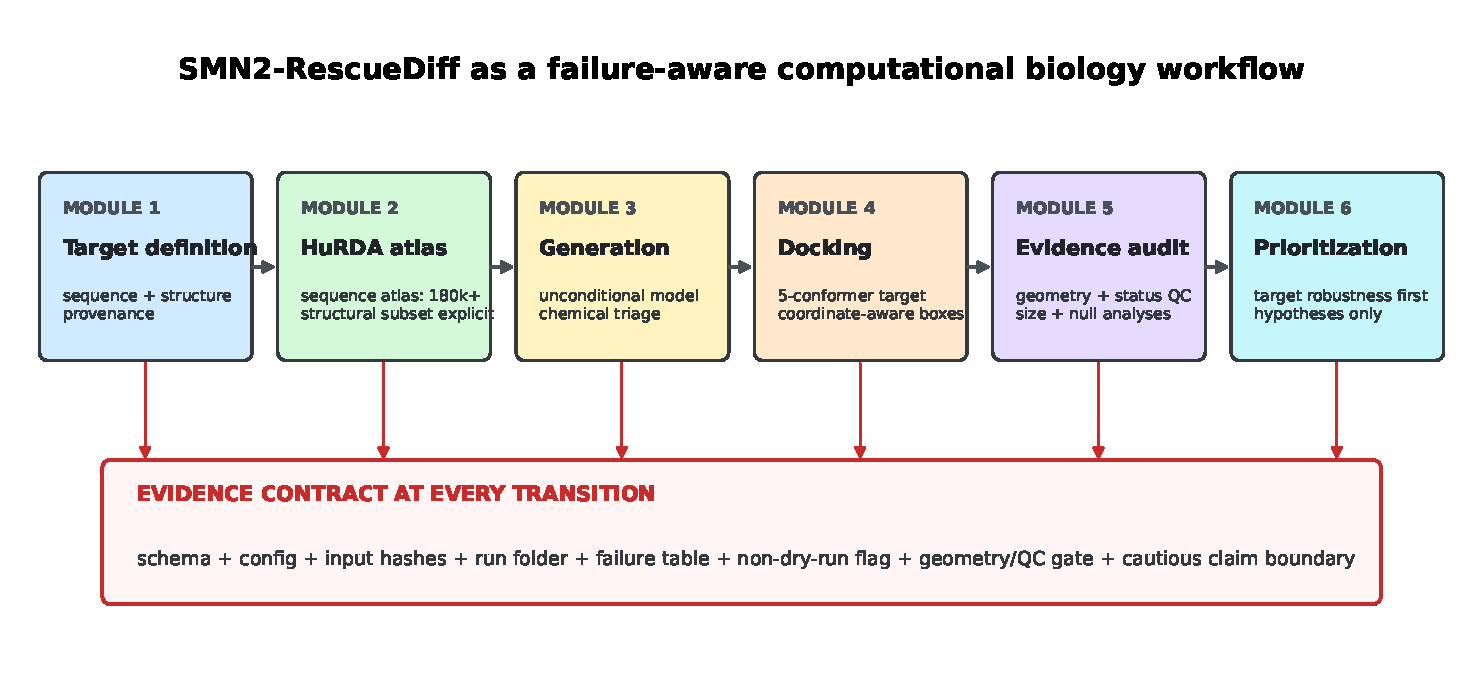
\includegraphics[width=\textwidth]{figures/Fig_pipeline_evidence_contracts.pdf}
\caption{SMN2-RescueDiff architecture. The contribution emphasized in
this revision is the horizontal evidence contract: data schemas,
configuration, provenance, failure records, score origin, geometry QC,
and claim boundaries accompany every stage.}
\label{fig:pipeline}
\end{figure*}

\begin{table}[!t]
\caption{Evidence-contract requirements}
\label{tab:contracts}
\centering
\footnotesize
\begin{tabular}{p{0.22\columnwidth}p{0.66\columnwidth}}
\toprule
Contract element & Required behavior \\
\midrule
Identity & Stable molecule, receptor, conformer, and run identifiers \\
Provenance & Input paths/hashes, source metadata, copied configuration \\
Execution & Engine, status, dry-run flag, seed, parameters, output path \\
Missingness & Failure reason retained; no silent score imputation \\
Geometry & Receptor/ligand format and coordinate-box coverage validated \\
Interpretation & Numeric output labeled as proxy, calibrated result, or audit-only \\
\bottomrule
\end{tabular}
\end{table}

\subsection{Module 1: \textit{SMN2} target definition}

Module 1 defined exon-7-centered windows from a configured genome and
annotation, converted DNA sequence to RNA, and emitted FASTA, feature,
and metadata files. It calculated nucleotide frequencies, GC content,
k-mer counts, simple splice-site/U1-complementarity features, and
distances from exon boundaries. These quantities define a reproducible
target profile; they are not evidence of small-molecule activity.

The structural target panel used the first five deposited models of the
8R62 solution-NMR ensemble. These are five conformations of one
risdiplam-associated RNA complex, not five independent biological
targets. This narrow ensemble probes local conformer sensitivity but
does not represent all accessible \textit{SMN2} RNA folds.

\subsection{Module 2: HuRDA sequence atlas and structural subset}

HuRDA-180K was designed as a sequence-level counter-screening resource.
It contains over 180,000 candidate motifs from 5$'$ and 3$'$ splice
sites, exon- and intron-adjacent windows, \textit{SMN2}-like sequences,
mutated/scrambled controls, and bias-matched transcript windows. Each
record has a conservative category label, sequence features, similarity
scores, and train/validation/test or holdout assignment.

The sequence atlas must not be confused with structural docking
coverage. One hundred motifs were prepared as predicted RNA receptors;
97 formed the common historical candidate matrix. Predicted structures
do not establish native folds, accessibility, expression, or binding.
The atlas supplies candidate decoys for staged experiments, not a
transcriptome-wide safety screen.

\subsection{Module 3: molecular generation and triage}

The production generator was a decoder-only Transformer trained
autoregressively on SELFIES tokens with causal masking. Training used
149,534 valid ChEMBL/ZINC-derived rows from 150,000 configured records.
The configured R-BIND and SMMRNA sources contributed zero rows to this
historical run. Known splicing modifiers were held out as benchmark
controls and were not used for model training. Exact upstream database
release identifiers and redistribution licenses could not be recovered
with sufficient certainty, an end-to-end reproducibility limitation.

Generated strings were converted to canonical SMILES with RDKit,
deduplicated at the canonical graph level, and filtered for molecular
weight, lipophilicity, hydrogen-bond counts, rotatable bonds, polar
surface area, Lipinski criteria, PAINS alerts, novelty, and a documented
synthetic-accessibility proxy. A fingerprint-based diversity selector
created the docking export. These are cheminformatic prioritization
features, not RNA-activity labels.

For a controlled baseline, the same configured training-source mixture
and requested sample count were supplied to a token 3-gram SMILES
generator. The comparison measures valid and filter-pass yield under
the two representations/architectures. It does not isolate every design
choice and is not an external biological benchmark.

\subsection{Module 4: target and decoy docking}

Ligands were prepared in SDF and PDB for inspection and converted with
Open Babel to PDBQT. Only an existing ligand PDBQT and receptor PDBQT
can enter AutoDock Vina. Missing PDBQT files produce an explicit failed
job. Target docking used identical Vina settings across the five target
conformers. All reported scientific scores have
\texttt{is\_dry\_run\_score=false}.

For molecule $i$ and target conformers $c=1,\ldots,5$, robustness
statistics were
\begin{equation}
 \bar E_i^T=\frac{1}{5}\sum_c E_{ic}^T, \quad
 E_{i,\mathrm{worst}}^T=\max_c E_{ic}^T,
\end{equation}
with lower Vina values considered more favorable within this protocol.
The primary ranking requires all five jobs and orders candidates by
$E_{i,\mathrm{worst}}^T$, then $\bar E_i^T$, then conformer range and
standard deviation. This prevents one unusually favorable conformer
from controlling advancement.

The original decoy implementation reused the target box for all
receptors. The corrected implementation supports
\texttt{per\_receptor\_bounds}: for receptor atom coordinates
$\mathbf{x}_{1},\ldots,\mathbf{x}_{n}$ and padding $p$, the box center
and size are
\begin{equation}
 \mathbf{c}=\frac{\min_j\mathbf{x}_j+\max_j\mathbf{x}_j}{2},\qquad
 \mathbf{s}=\max_j\mathbf{x}_j-\min_j\mathbf{x}_j+2p.
\end{equation}
A fixed box can alternatively be used only when its receptor atom
coverage exceeds a configured minimum. The current preset requires
complete receptor-specific coverage and writes a per-receptor box-QC
table before docking.

\subsection{Historical Module 5 scores and primary analysis rule}

The historical Stage C ranking was lexicographic and in practice was
controlled by a continuous target--decoy gap. SRSI was a separate
standardized weighted score that included target Vina score, the same
target score inside gap and contact-derived terms, chemical quality, and
penalties. They were not one rule. Because the decoy scores fail the
coordinate audit and target evidence was counted in correlated terms,
neither Stage C nor SRSI is the primary analysis here.

The SRSI is retained as a reproducibility artifact and labeled a
heuristic. Its former ``splicing-rescue proxy'' is renamed the
\emph{geometric contact proxy}. It used global atom-pair counts and
fixed fractional assignments rather than nucleotide-mapped functional
contacts; several terms were saturated or nearly constant. It has not
been calibrated against exon-7 inclusion and carries no mechanistic
interpretation. The primary rule in this paper is the prespecified
five-conformer target robustness ranking above.

\subsection{Post hoc falsification analyses}

For each historical decoy receptor, atom coordinates were compared with
the original target-centered box. We calculated receptor atom coverage,
exact-zero score fraction, receptor-level mean score, and Spearman
correlation between coverage and score. One-way variance decomposition
estimated the fraction of total score variance associated with receptor
or ligand identity. Historical scores were not modified.

To inspect exact zeros, 250 zero-score and 250 nonzero-score jobs were
sampled with seed 42. The minimum Euclidean distance between any ligand
pose atom and receptor atom was calculated. Sensitivity analyses
recomputed mean gaps after excluding zeros, conservative gaps after
removing the strongest one or three decoy receptors, and worst-decoy
statistics across 2,000 randomly sampled panels of 5, 10, 20, or 50
receptors. These analyses diagnose the historical experiment; they do
not repair it.

Molecular-size sensitivity used RDKit heavy-atom count and molecular
weight. A Vina ligand-efficiency descriptor was defined as
$-\bar E_i^T/N_i^{\mathrm{heavy}}$. A linear score-versus-weight model
provided a residual ranking. Neither is a binding free energy.

\subsection{Calibration and additional campaigns}

The docking protocol was evaluated on four deposited RNA--ligand
complexes: 8R62/risdiplam, 8R63/branaplam, 8R8P/SMN-CX, and 5KX9/a
ribocil analogue. Five seeds and retained modes distinguished sampling
from top-rank scoring. A rank-1 pose below 2~\AA{} was the prespecified
recovery criterion.

A 40-molecule by 20-receptor non-RNA campaign was also released with
all 800 scores, logs, poses, receptor inputs, and provenance. It tests
pipeline execution and provides an exploratory promiscuity audit.
Scores across heterogeneous proteins and RNA are not assumed to be
commensurate binding energies. Risdiplam and branaplam target scores are
released as held-out descriptive references. Their 2$\times$100 decoy
run shares the historical box defect and is audit-only.

\section{Results}

\subsection{Generation accounting and controlled baseline}

The production sampler requested 50,000 samples and emitted 49,660
unique valid strings. Canonicalization collapsed 171 strings onto an
already observed graph, leaving 49,489 unique canonical molecules.
Chemical filters rejected 9,012 unique molecules and retained 40,477;
the 9,183-row rejection table includes both those failures and the 171
canonical duplicates. Diversity selection exported 1,000 molecules
(Table~\ref{tab:generation}; Fig.~\ref{fig:generation}). This resolves
the previously ambiguous arithmetic and gives each percentage a named
denominator.

\begin{table}[!t]
\caption{Production generation flow}
\label{tab:generation}
\centering
\footnotesize
\begin{tabular}{lr}
\toprule
Stage & Count \\
\midrule
Samples requested & 50,000 \\
Unique valid strings emitted & 49,660 \\
Canonicalization collapses & 171 \\
Unique canonical molecules & 49,489 \\
Unique chemical-filter failures & 9,012 \\
Retained unique molecules & 40,477 \\
Total rejection records & 9,183 \\
Docking export & 1,000 \\
\bottomrule
\end{tabular}
\end{table}

\begin{figure*}[!t]
\centering
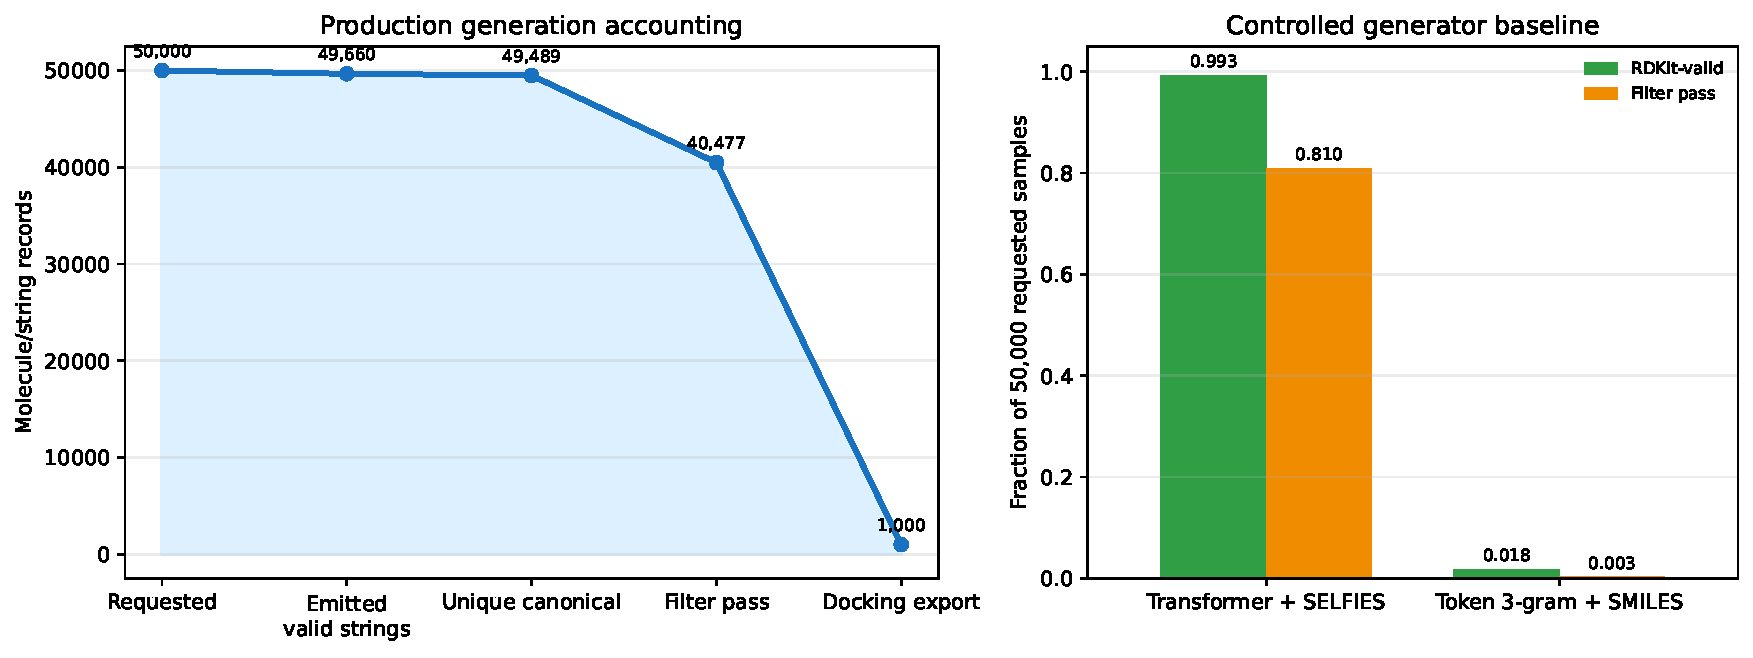
\includegraphics[width=0.94\textwidth]{figures/Fig_generation_and_baseline.pdf}
\caption{Left: mutually reconciled production-generation flow. Right:
controlled 50,000-sample engineering baseline. Transformer/SELFIES
produced 49,660 valid and 40,477 filter-pass records; token 3-gram/SMILES
produced 915 and 163. The comparison is not a biological validation.}
\label{fig:generation}
\end{figure*}

The 3-gram baseline produced 915 RDKit-valid records (1.83\% of
requested samples), 535 unique valid molecules, and 163 filter-pass
molecules (0.326\%). The production Transformer/SELFIES route produced
valid and filter-pass fractions of 99.32\% and 80.954\%, respectively.
Representation and architecture differ together, so this experiment
shows a practical yield advantage for the production route, not that a
specific neural component learned RNA recognition.

\subsection{Five-conformer target screen}

All 2,500 planned target jobs completed for 500 molecules and five 8R62
models. Across molecules, the median mean score was -7.193~kcal/mol and
the median worst-conformer score was -7.018~kcal/mol. MolGen\_038292 was
ranked first by the robustness rule, with a mean of -8.929, worst score
of -8.590, standard deviation 0.306, and range 0.776~kcal/mol
(Fig.~\ref{fig:target}). These numbers identify a reproducible Vina
ranking within one narrow receptor ensemble; they do not establish
binding.

\begin{figure}[!t]
\centering
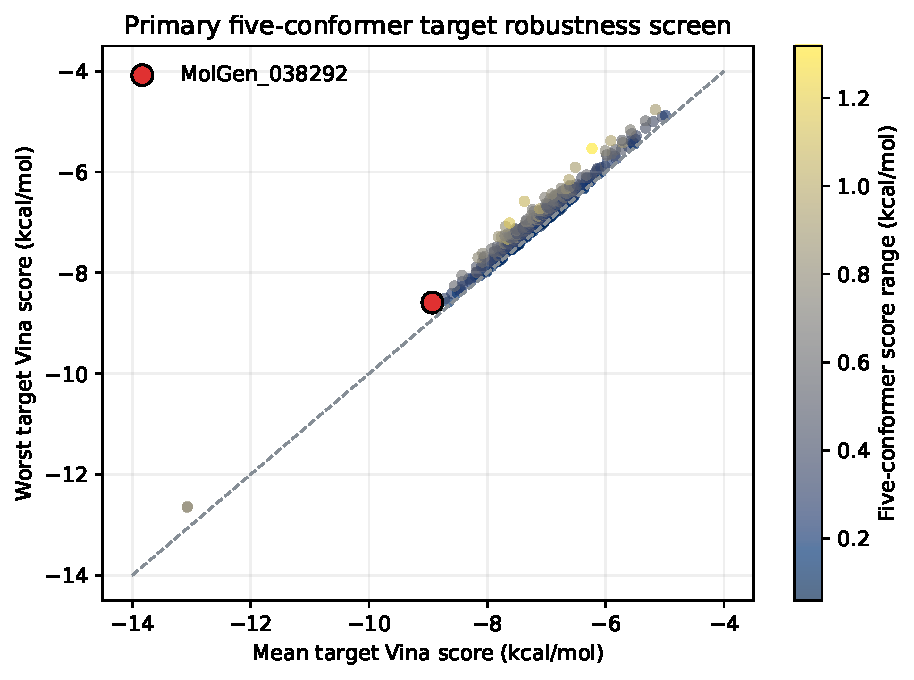
\includegraphics[width=\columnwidth]{figures/Fig_target_robustness.pdf}
\caption{Mean and worst-conformer target Vina scores for 500 molecules.
Color is the five-conformer range. Advancement requires all five jobs
and prioritizes the worst score before the mean.}
\label{fig:target}
\end{figure}

The previous matched-control analysis selected a top 40 using a rule
containing target score and then tested target score. Its mean enrichment
was 0.729~kcal/mol, but a target-only top 40 produced 1.016~kcal/mol and
overlapped 35 of 40 molecules. Moreover, 400 candidate--control
assignments reused 183 controls. The result is therefore reported only
as within-cohort selection behavior. It is not independent evidence of
prediction, SRSI utility, or selectivity.

\subsection{Structural decoy audit falsifies the historical inference}

The historical decoy table contains 14,259 completed, non-dry-run Vina
rows for a complete 147$\times$97 matrix. Completeness did not imply
valid comparison. Eighty-one of 97 receptors had less than 10\% of atoms
inside the fixed target box. Coverage correlated strongly with receptor
mean score ($\rho=-0.8469$, $p=8.36\times10^{-28}$;
Fig.~\ref{fig:geometry}). Receptors below 10\% coverage averaged
-1.193~kcal/mol, whereas the remainder averaged -6.886~kcal/mol.
Receptor identity explained 98.83\% of score variance and ligand
identity 0.132\% (Table~\ref{tab:audit}).

\begin{figure}[!t]
\centering
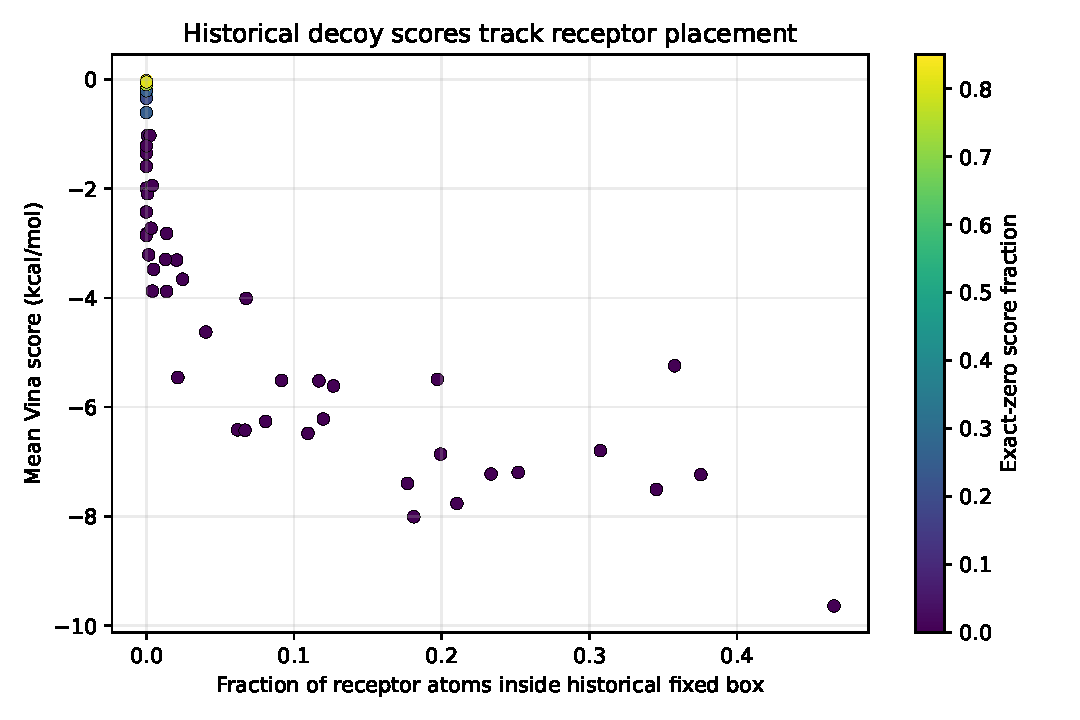
\includegraphics[width=\columnwidth]{figures/Fig_decoy_geometry_bias.pdf}
\caption{Historical decoy scores track the fraction of each receptor
inside the target-centered box. Color denotes exact-zero score
frequency. This geometry dependence invalidates target--decoy
selectivity interpretation of the campaign.}
\label{fig:geometry}
\end{figure}

\begin{table}[!t]
\caption{Historical decoy falsification audit}
\label{tab:audit}
\centering
\footnotesize
\begin{tabular}{lr}
\toprule
Diagnostic & Result \\
\midrule
Completed historical jobs & 14,259 \\
Receptors / ligands & 97 / 147 \\
Receptors with $<10\%$ atoms in box & 81 \\
Exact-zero scores & 4,815 (33.77\%) \\
Coverage--mean-score Spearman $\rho$ & -0.8469 \\
Variance associated with receptor & 98.83\% \\
Variance associated with ligand & 0.132\% \\
Strongest receptor for all ligands & HuRDA\_000041 \\
All observed decoy weights & 1.0 \\
\bottomrule
\end{tabular}
\end{table}

Exact zeros were structural warning signals, not missing values. In the
seeded pose sample, zero-score poses had a median minimum ligand--receptor
distance of 32.65~\AA{}, compared with 2.58~\AA{} for nonzero poses.
The median historical mean gap decreased from 5.590 to
4.573~kcal/mol when exact zeros were excluded. HuRDA\_000041 was the
strongest-scoring decoy for all 147 ligands. Removing it changed the
median conservative gap from -1.950 to -0.502~kcal/mol and made 12 of
147 gaps nonnegative; removing the three strongest receptors produced a
median of -0.098 and 54 nonnegative gaps. Worst-decoy behavior also
changed substantially with random panel size (Fig.~\ref{fig:panel}).

\begin{figure}[!t]
\centering
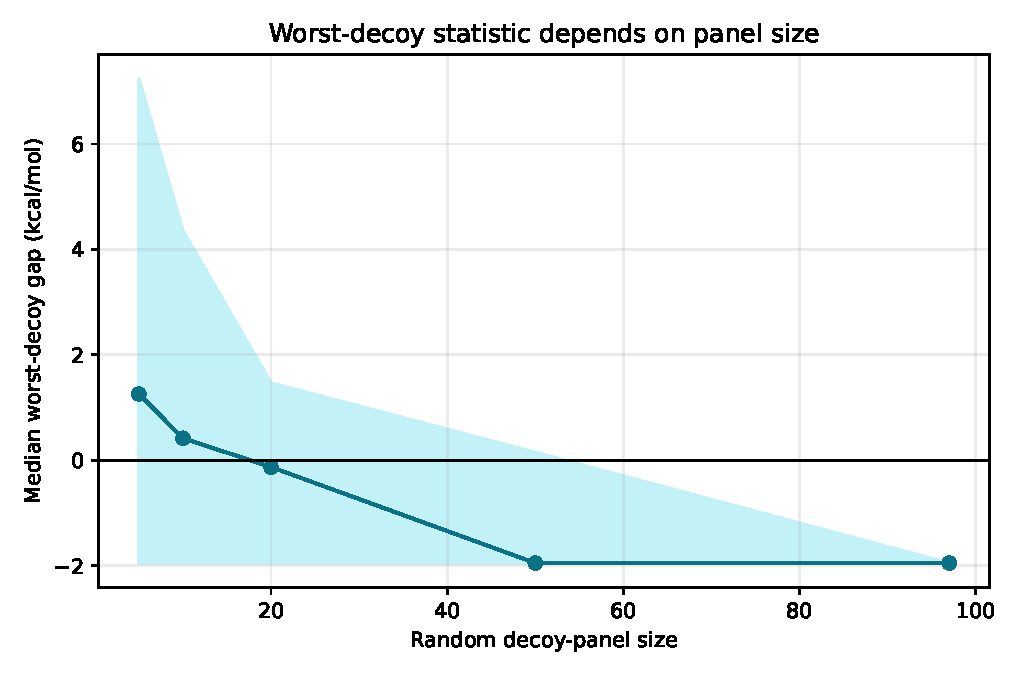
\includegraphics[width=\columnwidth]{figures/Fig_decoy_panel_sensitivity.pdf}
\caption{Historical worst-decoy statistic as a function of randomly
sampled panel size. The dependence is descriptive because the underlying
fixed-box experiment is invalid for selectivity inference.}
\label{fig:panel}
\end{figure}

All historical decoy weights were 1.0, so the former ``biologically
weighted'' gap was an unweighted mean. The previously reported finding
that all conservative gaps were negative cannot be interpreted as true
poor selectivity: it is dominated by receptor placement. Conversely,
the favorable mean gaps cannot be interpreted as selectivity either.
Both directions of biological inference are withdrawn pending corrected
receptor-specific redocking.

\subsection{Corrected candidate descriptors and size sensitivity}

RDKit recomputation corrected MolGen\_038292 to molecular weight
377.448~Da, QED 0.8563, cLogP 2.7055, two donors, six acceptors, three
rotatable bonds, tPSA 79.38~\AA$^2$, and 28 heavy atoms. Historical
copy stating 504~Da and QED 0.498 was wrong. The corrected historical
stronger-decoy quantity is 1/97 = 0.010309 as a fraction, or 1.0309\%;
because the decoy campaign is invalid, even the corrected value is
audit-only.

Mean target score correlated with molecular weight at
$\rho=-0.5054$ ($p=9.06\times10^{-34}$; Fig.~\ref{fig:size}).
MolGen\_038292 had Vina ligand efficiency 0.3189 and ranked 136 of 500
by that descriptor. Its molecular-weight-adjusted score residual was
-1.344~kcal/mol, rank 3 of 500. Thus its target rank is not explained
only by molecular weight, but raw Vina score cannot be called a stronger
binding affinity or clinical advantage.

\begin{figure}[!t]
\centering
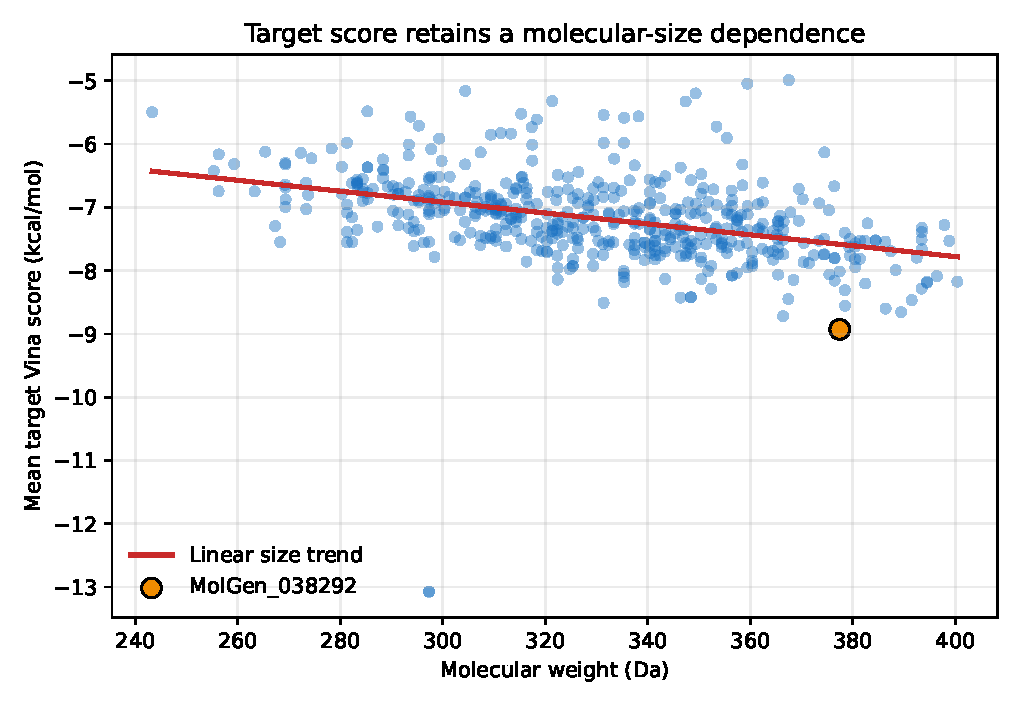
\includegraphics[width=\columnwidth]{figures/Fig_target_size_confounding.pdf}
\caption{Molecular weight retains a substantial association with mean
target Vina score. The line is a post hoc linear trend used for residual
sensitivity, not an affinity calibration.}
\label{fig:size}
\end{figure}

Risdiplam and branaplam were held out from training. A separately
released real Vina target run produced scores of -8.591 and
-8.321~kcal/mol, respectively, against one prepared target receptor.
Those values are descriptive references under a different receptor
design than the five-conformer candidate summary. No statement that a
generated molecule is clinically or biophysically superior is made.

\subsection{Calibration and released auxiliary campaigns}

Redocking was mixed (Table~\ref{tab:redock}; Fig.~\ref{fig:redock}).
Branaplam achieved a rank-1 pose at 1.307~\AA{} from deposited model 1;
risdiplam, SMN-CX, and the ribocil analogue had rank-1 RMSDs of 12.587,
7.169, and 6.173~\AA{}. Lower-ranked modes reached 2.478~\AA{} for
risdiplam and 1.856~\AA{} for SMN-CX, distinguishing sampling from
ranking failure. One of four rank-1 successes is weak calibration and
does not validate prospective screening.

\begin{table}[!t]
\caption{RNA--ligand redocking calibration}
\label{tab:redock}
\centering
\scriptsize
\begin{tabular}{lrrr}
\toprule
Ligand & Rank-1 RMSD & Best mode RMSD & Rank-1 $<2$~\AA{} \\
\midrule
Risdiplam & 12.587 & 2.478 & No \\
SMN-CX & 7.169 & 1.856 & No \\
Ribocil analogue & 6.173 & 4.384 & No \\
Branaplam & 1.307 & 1.137 & Yes \\
\bottomrule
\end{tabular}
\end{table}

\begin{figure}[!t]
\centering
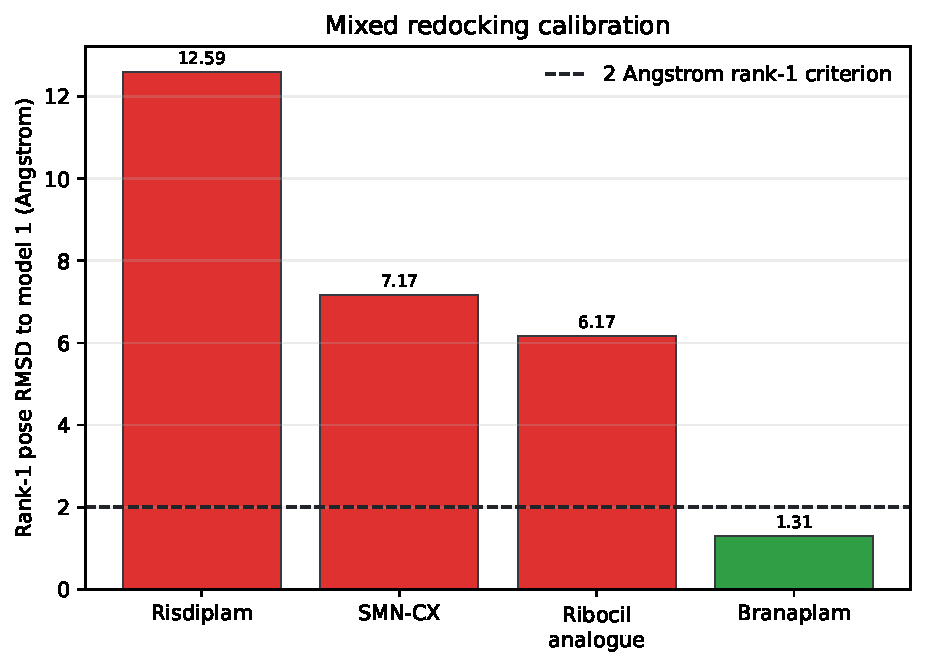
\includegraphics[width=\columnwidth]{figures/Fig_redocking_calibration.pdf}
\caption{Rank-1 pose RMSD for four deposited RNA--ligand complexes. The
dashed line is the prespecified 2~\AA{} criterion.}
\label{fig:redock}
\end{figure}

The previously uncheckable cross-target claim is now supported by an
800-row table: 40 molecules, 20 receptors, 800 completed real Vina jobs,
with all logs and poses released. This closes an artifact gap but does
not validate cross-class score comparability. The complete risdiplam/
branaplam 2$\times$100 campaign is also released; its decoy portion is
quarantined because it shares the fixed-box defect.

\section{Discussion}

\subsection{The computational-biology innovation}

The strongest outcome of this project is not that a molecule ``won'' a
docking table. It is that the pipeline retained enough structure to
show why an apparently complete selectivity result was invalid. The
original matrix had real Vina jobs, valid PDBQT inputs, no imputation,
and complete molecule--decoy coverage. Conventional completeness checks
therefore passed. The missing check was geometric: receptors generated
in different coordinate frames cannot inherit a target-centered search
box. Once box coverage was measured, the source of the signal became
quantifiable rather than speculative.

This suggests a broader TCBB design principle. In multistage workflows,
schema validation alone is insufficient; evidence contracts must include
domain invariants. For docking, those invariants include coordinate
frames, atom coverage, receptor preparation, and score origin. For
generation, they include canonicalization denominators and held-out
benchmarks. For ranking, they include independence between the selection
criterion and validation endpoint. Encoding such checks makes failure a
first-class, reproducible output.

The new Module 4 behavior operationalizes that principle. Each decoy can
receive a box derived from its own receptor bounds, and a fixed box must
pass a configurable coverage threshold. The run writes receptor-specific
box QC alongside scores. This does not guarantee biological accuracy,
but it prevents the exact coordinate mismatch found here. The same
principle applies beyond docking: downstream modules should reject an
upstream artifact that cannot satisfy its scientific preconditions.

\subsection{What succeeded, and what did not}

The workflow succeeded as software and as an audit system. It trained
and sampled a production generator, reconciled generation denominators,
outperformed a simple baseline on usable yield, completed a five-model
target campaign, ranked without a best-conformer shortcut, released a
previously missing 800-job campaign, and surfaced the structural-decoy
failure. These are meaningful computational-engineering results.

The study did not demonstrate predictive RNA selectivity or exon-7
rescue. Historical mean and conservative gaps are unusable for that
purpose. Target-only matched-control behavior is partly selected by
construction. SRSI combines correlated, uncalibrated terms and is a
heuristic. Redocking is weak at rank 1. AutoDock Vina was parameterized
primarily for protein--ligand systems, and its values are comparative
scores rather than measured free energies~\cite{trott2010,eberhardt2021,
agarwal2023,gunasinghe2024}.

This candid boundary strengthens rather than erases the pipeline's
contribution. A computational platform intended for iterative science
must support negative audits and claim withdrawal, not only successful
runs. Preserving the historical scores alongside their falsification
analysis makes the error inspectable and prevents retroactive data
cleaning from disguising it.

\subsection{Ranking implications}

Target-conformer robustness is the only primary ranking in this
revision. It is intentionally modest: it prioritizes molecules whose
Vina scores are consistently favorable across five models of one RNA
ensemble. It does not use the invalid decoy panel, saturated contact
terms, or target-score enrichment as independent validation.

The historical Stage C and SRSI outputs remain useful for software
regression and ablation, but not for biological inference. Future
ranking weights should be learned or selected using independent labels,
and evaluation should compare the full rule with target-only, size-aware,
and simple cheminformatic baselines on held-out compounds and scaffolds.
Until then, ``geometric contact proxy'' is the maximum defensible label
for the former rescue feature.

\subsection{Limitations and required validation}

This study has several nontrivial limitations.

First, no direct RNA-binding assay, cell-based exon-7 inclusion assay,
toxicity measurement, pharmacokinetic result, or animal experiment was
performed. The outputs are hypotheses for prospective testing.

Second, corrected receptor-specific HuRDA docking is configured but not
completed in this report. No corrected selectivity number is substituted
for the invalid historical one. A staged campaign should first test a
small prespecified panel, inspect poses and box coverage, then expand to
500--1,000 hard decoys only if QC passes. Docking all 180,000 sequence
motifs would conflate sequence coverage with unsupported structure
prediction and waste computation.

Third, the target ensemble is the first five 8R62 NMR models associated
with a ligand-bound complex. Alternative RNA folds, preparation choices,
protonation/charge models, water/ion treatment, and box definitions may
change ranks. The first five models are not independent targets.

Fourth, four redocking complexes are too few to estimate generalization.
A prespecified benchmark of at least 20--30 structurally diverse
RNA--ligand complexes, appropriate nonbinders, multiple folds, and both
pose and binder-ranking metrics is required. RNA-aware rescoring should
be tested against Vina. These experiments are outstanding; no surrogate
labels were fabricated.

Fifth, the generator baseline is deliberately simple. It combines a
different representation and architecture and does not compare against
matched GRU, random-library, or database-retrieval baselines. The
production generator was not trained on RNA-focused rows and is not
target conditioned. Its advantage here is usable sample yield, not
demonstrated RNA-ligand learning.

Sixth, exact ChEMBL/ZINC releases, retrieval dates, and redistribution
licenses for the historical subset could not be reconstructed. The
checkpoint, tokenizer, configuration, source accounting, and hashes are
released, but the third-party corpus is not redistributed. This prevents
full regeneration from the release alone.

Finally, 190 rows in the merged target table have a blank legacy engine
field despite completed non-dry-run provenance elsewhere. They were not
silently relabeled. Future merges must enforce non-null engine metadata.

\subsection{Prospective validation plan}

A defensible next study has three locked stages. Stage 1 will run the
receptor-specific-box HuRDA panel and reject any receptor that fails atom
coverage, typing, or pose-contact QC. Stage 2 will benchmark Vina and at
least one RNA-aware reranker on a predeclared external complex/binder
set with scaffold-separated splits. Stage 3 will test a small,
chemically diverse candidate set using direct binding and \textit{SMN2}
exon-7 inclusion assays, with risdiplam and branaplam as held-out
reference controls. Only those data could support a rescue or therapeutic
claim.

\section{Conclusion}

SMN2-RescueDiff demonstrates a reproducible, failure-aware architecture
for RNA-ligand prioritization. The pipeline generated and triaged a large
molecular cohort, completed a robust five-conformer target screen, and
published run-level evidence across generation, docking, redocking, and
auxiliary campaigns. More importantly, it exposed that a complete real-
Vina decoy matrix was dominated by an incompatible search box, quantified
the effect, preserved the failed evidence, and changed the software so
that the same error is rejected prospectively.

The scientific claim is deliberately narrow. MolGen\_038292 is a
computationally prioritized target-docking hypothesis, not a drug.
Historical HuRDA scores do not establish selectivity, SRSI does not
establish splicing rescue, and mixed redocking does not validate the
ranker. The contribution to computational biology is the auditable
methodology that makes those boundaries visible and enforceable. In a
field where multistage workflows can amplify one hidden assumption into
a persuasive final rank, detecting and containing invalid evidence is
itself a necessary form of computational rigor.

\section*{Acknowledgments}

The author used ChatGPT, Claude, Codex, and Grammarly for code review,
repository auditing, figure layout, and manuscript revision. These tools
did not generate the historical docking calculations. Numerical claims
in this revision were recomputed from released tables or logs, and no
missing score was invented or imputed. The author reviewed the complete
text and takes responsibility for its claims. The author thanks
Dr.~Joy Li (Duke University) for mentorship.

\section*{Code and Data Availability}

The source and evidence release are available at
\url{https://github.com/}\url{sakshams-cyber/SMN2-RescueDiff}. The
audited evidence tree is immutable at commit \texttt{5e24251} under
\texttt{reproducibility/tcbb\_2026}. The
\texttt{reproducibility/tcbb\_2026} directory contains target and
historical decoy inputs/scores, failure records, audit tables, redocking,
the complete 40$\times$20 campaign, benchmark-control v2 files, the
production checkpoint/tokenizer/configuration, the 50,000-sample
baseline, source manifests, and checksum files. The
review-response ledger in the \texttt{docs} directory maps each
evaluator request to an implemented correction, withdrawn claim,
partial release, or outstanding experiment. The Overleaf package
contains this source, all figure inputs, generated figures, a change
report, and a reproducible build guide.

\section*{Declarations}

\textit{Ethical approval:} Not applicable. This computational study used
no human participants, identifiable human data, or animal subjects.

\begin{thebibliography}{19}

\bibitem{aslesh2022}
T. Aslesh and T. Yokota, ``Restoring SMN expression: An overview of the
therapeutic developments for the treatment of spinal muscular
atrophy,'' \emph{Cells}, vol. 11, no. 3, p. 417, 2022.

\bibitem{chong2021}
L. C. Chong, G. Gandhi, J. M. Lee, W. W. Y. Yeo, and S.-B. Choi,
``Drug discovery of spinal muscular atrophy from the computational
perspective: A comprehensive review,'' \emph{Int. J. Mol. Sci.},
vol. 22, no. 16, p. 8962, 2021.

\bibitem{warner2018}
K. D. Warner, C. E. Hajdin, and K. M. Weeks, ``Principles for targeting
RNA with drug-like small molecules,'' \emph{Nat. Rev. Drug Discov.},
vol. 17, pp. 547--558, 2018.

\bibitem{childs2022}
J. L. Childs-Disney \emph{et al.}, ``Targeting RNA structures with small
molecules,'' \emph{Nat. Rev. Drug Discov.}, vol. 21, pp. 736--762, 2022.

\bibitem{haga2023}
C. L. Haga and D. G. Phinney, ``Strategies for targeting RNA with small
molecule drugs,'' \emph{Expert Opin. Drug Discov.}, vol. 18,
pp. 135--147, 2023.

\bibitem{wen2026}
Y. Wen, Y. Han, and D. Wang, ``Overcoming shortcut learning in
RNA-small molecule modeling via bias-matched decoys and structure-aware
network design,'' \emph{J. Chem. Inf. Model.}, vol. 66,
pp. 6403--6417, 2026.

\bibitem{agarwal2023}
R. Agarwal, R. Rajeshwar T., and J. C. Smith, ``Comparative assessment
of pose prediction accuracy in RNA--ligand docking,'' \emph{J. Chem.
Inf. Model.}, vol. 63, pp. 7444--7452, 2023.

\bibitem{gunasinghe2024}
K. K. J. Gunasinghe \emph{et al.}, ``Can current molecular docking
methods accurately predict RNA inhibitors?,'' \emph{J. Chem. Inf.
Model.}, vol. 64, pp. 5954--5963, 2024.

\bibitem{zdrazil2024}
B. Zdrazil \emph{et al.}, ``The ChEMBL database in 2023,''
\emph{Nucleic Acids Res.}, vol. 52, pp. D1180--D1192, 2024.

\bibitem{irwin2020}
J. J. Irwin \emph{et al.}, ``ZINC20---A free ultralarge-scale chemical
database for ligand discovery,'' \emph{J. Chem. Inf. Model.}, vol. 60,
pp. 6065--6073, 2020.

\bibitem{krenn2020}
M. Krenn \emph{et al.}, ``Self-referencing embedded strings (SELFIES):
A 100\% robust molecular string representation,'' \emph{Mach. Learn.
Sci. Technol.}, vol. 1, p. 045024, 2020.

\bibitem{baell2010}
J. B. Baell and G. A. Holloway, ``New substructure filters for removal
of pan assay interference compounds,'' \emph{J. Med. Chem.}, vol. 53,
pp. 2719--2740, 2010.

\bibitem{bickerton2012}
G. R. Bickerton \emph{et al.}, ``Quantifying the chemical beauty of
drugs,'' \emph{Nat. Chem.}, vol. 4, pp. 90--98, 2012.

\bibitem{trott2010}
O. Trott and A. J. Olson, ``AutoDock Vina: Improving the speed and
accuracy of docking,'' \emph{J. Comput. Chem.}, vol. 31,
pp. 455--461, 2010.

\bibitem{eberhardt2021}
J. Eberhardt, D. Santos-Martins, A. F. Tillack, and S. Forli,
``AutoDock Vina 1.2.0,'' \emph{J. Chem. Inf. Model.}, vol. 61,
pp. 3891--3898, 2021.

\bibitem{olivecrona2017}
M. Olivecrona \emph{et al.}, ``Molecular de-novo design through deep
reinforcement learning,'' \emph{J. Cheminformatics}, vol. 9, p. 48,
2017.

\bibitem{xi2024}
W. Xi \emph{et al.}, ``An interpretable deep learning model predicts
RNA--small molecule binding sites,'' \emph{Future Gener. Comput. Syst.},
vol. 159, pp. 557--566, 2024.

\bibitem{zhou2024}
Y. Zhou and S.-J. Chen, ``Advances in machine-learning approaches to
RNA-targeted drug design,'' \emph{Artif. Intell. Chem.}, vol. 2,
p. 100053, 2024.

\bibitem{rezaei2022}
M. A. Rezaei, Y. Li, D. Wu, X. Li, and C. Li, ``Deep learning in drug
design: Protein-ligand binding affinity prediction,'' \emph{IEEE/ACM
Trans. Comput. Biol. Bioinform.}, vol. 19, pp. 407--417, 2022.

\end{thebibliography}

\begin{IEEEbiographynophoto}{Saksham Srivastava}
is a student at Saint Francis High School, Mountain View, CA, USA. His
interests include computational biology, RNA-targeted molecular design,
and reproducible scientific software.
\end{IEEEbiographynophoto}

\end{document}
